\documentclass[a4paper,12pt]{article}

\usepackage[top=3cm, bottom=2cm, left=3cm, right=2cm]{geometry}
\usepackage[utf8]{inputenc}
\usepackage[portuguese]{babel}
\usepackage{booktabs}
\usepackage{multirow}
\usepackage{hyperref}
\usepackage{graphicx}
\usepackage{longtable}
\usepackage{verbatim}
\usepackage{url}
\usepackage{morefloats}
\usepackage{xcolor}
\usepackage{fancyvrb}

\usepackage{float}
\floatstyle{ruled}
\newfloat{program}{thp}{lop}
\floatname{program}{Log}
\newfloat{config}{thp}{lop}
\floatname{config}{Configuração}

\title{Serviços de Rede e de Sistema \\
Desenhar e correr um serviço de E-mail}

\author{André Fernandes (ei03107) \and Miguel Gomes (ei07075) \and Pedro Batista (ext10392)}

\begin{document}

\maketitle
\tableofcontents

\section{Topologia}


Em virtude da configuração DNS do laboratório estar {\bf incorrecta} decidimos 
mudar a topologia da rede conforme a figura \ref{fig:topologia}.
Esta alteração deveu-se ao facto de nem a máquina denominada por carvoeiro no 
guião (192.168.109.2), nem as máquinas com os IP 193.136.28.10 e 172.16.2.2 
presentes na rede, constarem de serviços DNS que conhecessem, simultaneamente,
os registo MX e A dos GNUs.

Mais especificamente, os serviços DNS do carvoeiro e da máquina 172.16.2.2 
conheciam o registo MX, mas não conhecia o endereço dos GNUs. Já o 
serviço DNS da máquina 193.136.28.10 conhecia os endereços dos GNUs mas 
não conhecia os registos MX.

Estas afirmações podem ser confirmadas pelos logs \ref{log:carvoeiromx}, 
\ref{log:carvoeiroa}, \ref{log:193a}, \ref{log:193mx}, \ref{log:172mx}
e \ref{log:172a}.

Embora a topologia implementada ter sido diferente do guião achámos que a
topologia não foi alterada signitivamente face ao objectivo trabalho proposto.

O trabalho realizado diferiu, essencialmente, em dois aspectos. Em primeiro
lugar, com o facto dos computadores estarem ligados directamente ao mesmo
switch. E em segundo, pelo domínio \emph{psb.com} ter sido configurado
numa máquina que chamámos de ``pa'' e que serviu como cliente
pop3 e imap.

\begin{figure}[htp]
	\begin{center}
		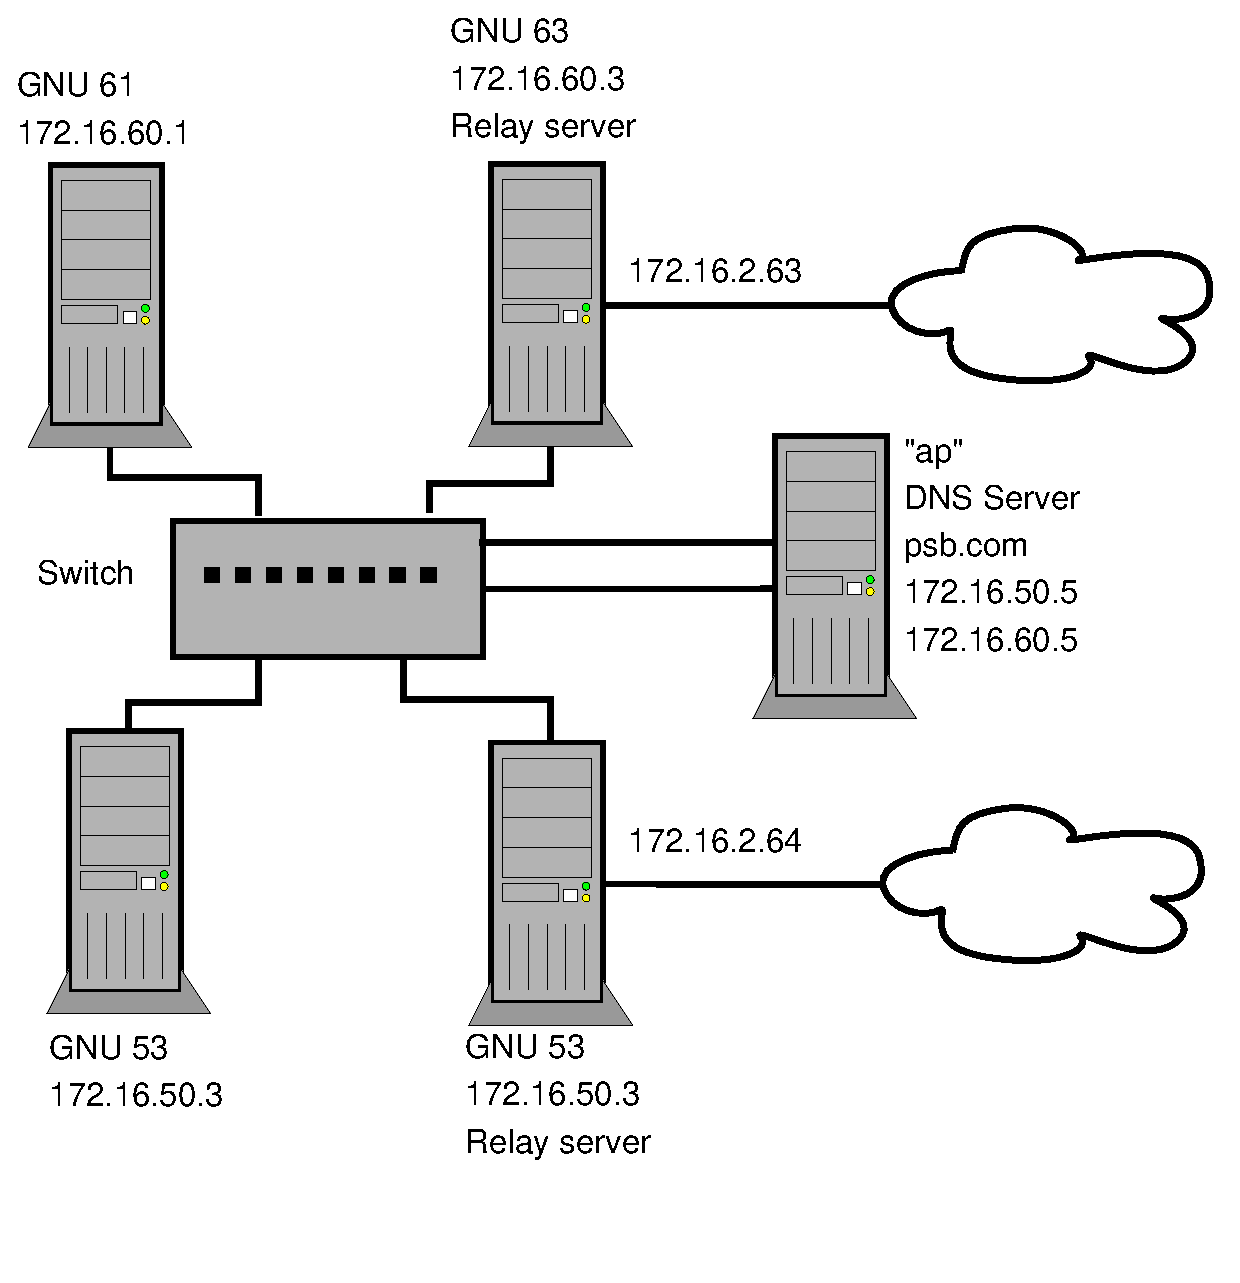
\includegraphics[height=6in]{topologia}
	\end{center}
	\caption{Topologia de rede implementada.}
	\label{fig:topologia}
\end{figure}

\begin{program}
	\verbatiminput{carvoeiro_mx}
  \caption{Pergunta ao carvoeiro sobre o registo MX da bancada6.}
	\label{log:carvoeiromx}
\end{program}

\begin{program}
	\verbatiminput{carvoeiro_a}
  \caption{Pergunta ao carvoeiro sobre o registo do GNU63.}
	\label{log:carvoeiroa}
\end{program}

\begin{program}
	\verbatiminput{193_mx}
  \caption{Pergunta à máquina 193.136.28.10 sobre o registo MX da bancada6.}
	\label{log:193mx}
\end{program}

\begin{program}
	\verbatiminput{193_a}
  \caption{Pergunta à máquina 193.136.28.10 sobre o registo do GNU63.}
	\label{log:193a}
\end{program}

\begin{program}
	\verbatiminput{172_mx}
  \caption{Pergunta à máquina 172.16.2.2 sobre o registo MX da bancada6.}
	\label{log:172mx}
\end{program}

\begin{program}
	\verbatiminput{172_a}
  \caption{Pergunta à máquina 172.16.2.2 sobre o registo do GNU63.}
	\label{log:172a}
\end{program}


\section{Configurações}

Os ficheiros das configurações encontram-se em anexo no arquivo ``conf''.
Dentro deste arquivo encontram-se pastas com o nome ``gXY'' com os ficheiros
de configuração para cada ``GNUXY''. Adicionalmente, encontra-se ainda um
arquivo com o nome ``pa'' com as configurações do servidor DNS presente na 
figura \ref{fig:topologia}.

\subsection{DNS}

A configuração \ref{conf:dns} mostra o registo DNS para a zona psb.com.
Observamos que como esperado os registros MX apontam para endereços válidos
desse domínio. Idealmente um servidor com views deveria ser implementado, isto
é, os servidores IMAP e POP3 só seriam observados dentro de cada bancada, já os
para os servidores de relay respostas diferentes deferiam ser encaminhadas se a
query fosse feita internamente ou do exterior.
Porém por questões de simplicidade não entramos a esse nível de detalhamento na
configuração.

\begin{config}
	\verbatiminput{conf/pa/psb.com.zone}
  \caption{Registo DNS para a zona psb.com.}
	\label{conf:dns}
\end{config}


\section{Registo de Logs}

Com o objectivo de registar o tráfego completo da rede configurámos uma porta
do switch como uma porta SPAN (Switched Port Analyzer) por forma a escutar todo
o tráfego da rede no Wireshark.
Uma vez que os arquivos das capturas são de grande dimensão decidímos anexar 
ao relatório um arquivo com todos estes registos com o nome de ``wireshark''. 
A sessões encontram-se organizadas como se segue:

\begin{itemize}
	\item Sessão 1 - Tráfego de SMTP dentro da bancada 6.
	\item Sessão 2 - Tráfego de SMTP da bancada 6 para a bancada 5.
	\item Sessão 3.1 - Tráfego POP3.
	\item Sessão 3.2 - Tráfego POP3 SSL.
	\item Sessão 4.1 - Tráfego IMAP.
	\item Sessão 4.2 - Tráfego IMAP SSL.
	\item Sessão 5.1 - Mail do user1 da bancada 6 para o user2 da bancada 6.
	\item Sessão 5.2 - Mail do user2 da bancada 6 para o netedu da bancada 6.
	\item Sessão 5.3 - Mail do netedu da bancada 6 para o user1 da bancada 6.
	\item Sessão 5.4 - Mail do user1 da bancada 5 para o user1 da bancada 6.
	\item Sessão 5.5 - Mail do user1 da bancada 5 para o user2 da bancada 6.
	\item Sessão 5.6 - Mail do user1 da bancada 5 para o netedu da bancada 6.
\end{itemize}

Em anexo no relatório, estão registada todas as sessões à excepção das
sessões 5.

\section{Análise de resultados}

\subsection{Sessão 1}

Nesta sessão podemos observar, o início do handshake TCP entre o cliente
e o servidor no pacote número 17 e o estabelecimento da conversa SMTP
no pacote 27. O envio da mensagem SMTP própriamente dita é iniciada no pacote
31 com a mensagem ``EHLO''. Posteriormente seguida por uma mensagem enviada
com o remetente do e-mail numa mensagem ``MAIL FROM'' no pacote 37, pelo 
destinatário numa mensagem ``RCPT TO'' no pacote 40, por uma mensagem ``DATA'' 
no pacote 45 e pelo conteúdo do e-mail num pacote IMF com o número 49. Após
esta troca de mensagens o protocolo STMP termina a comunicação com o pacote 55 e
o protocolo TCP termina a comunicação com o pacote 64.

Já no que diz respeito ao download dos e-mails via POP3, podemos observar
o handshake TCP inicial a partir do pacote 262 e o início da sessão POP3
com um ``OK Hello there''. Após o qual podemos observar a autenticação
POP3 que é conseguida com a mensagem ``OK logged in'' no pacote 284. Após este
pacote é possível observar o processo de sincronização das mensagens
locais com as presentes no servidor. E finalmente, o término da sessão POP3
e posterior fecho da sessão TCP.

\subsection{Sessão 2}

Nesta sessão, o user1 da bancada 6 enviou uma mensagem ao user2 da bancada 5.
Como tal, o utilizador user1 enviou um e-mail para o serviço Postfix do
GNU61, que encaminhou o e-mail para o relay do GNU63,
que por sua vez reencaminhou o e-mail para o GNU64 via exterior, que serviu de relay
e entregou o e-mail no seu destino final no serviço Postfix do GNU53.

Uma das formas possíveis para monitorar o trajecto da mensagem de e-mail é,
por exemplo, seguir os pacotes IMF com o conteúdo do e-mail trocados nestas 
máquinas. Os pacotes referentes às trocas das mensagens IMF são:
\begin{itemize}
	\item Pacote 108 - E-mail trocado entre ``pa'' e o GNU61.
	\item Pacote 657 - E-mail trocado entre GNU61 e GNU63.
	\item Pacote 1103 - E-mail trocado entre GNU63 e GNU54.
	\item Pacote 1155 - E-mail trocado entre GNU54 e GNU53.
\end{itemize}

Como se pode observar o GNU61, não conseguiu comunicar diretamente com o mundo 
exterior, o GNU61 teve que usar o relay GNU63, para o fazer. Da mesma forma, o
GNU53 não pode ser acedido do exterior diretamente, teve de ser alcançado
por intermédio do relay GNU54. O que faz com que o requisito da utilização
dos relays do trabalho prático ter sido alcançado.

\subsection{Sessão 3.1}

Esta sessão foi em tudo similar à Sessão 1 registada.

\subsection{Sessão 3.2}

Comparativamente à Sessão 1, em que foi possível observar uma sessão POP3 sem
encriptação, nesta sessão não foi possível observar o conteúdo dos pacotes POP3
no Wireshark. Aqui os pacotes apareceram com a mensagem ``Application
Data'' por terem sido encriptados e não terem sido reconhecidos como
uma comunicação numa sessão POP3 válida.

\subsection{Sessão 4.1}



\subsection{Sessão 4.2}

Á semelhança do que se passou com a Sessão 3.2, correspondente à comunicação
POP3 sobre SSL, nesta sessão não foi possível identificar a comunicação IMAP
identificada na Sessão 4.1 devido à encriptação dos dados.

\section{Conclusão}

Neste trabalho foi possível comprovar a utilização do protocolo SMTP no 
envio de e-mails para o serviço Postfix. E, quase em simultâneo, verificar 
a utilização dos protocolos POP3 e IMAP no download de e-mails do 
serviço Postfix. Bem como as suas principais diferenças.

No protocolo POP3 sempre que é lido um e-mail do servidor o mesmo é
apagado do servidor. Por contraste, no protocolo IMAP isto pode não se passar.

Também observámos a forma como os diversos serviços de SMTP colaboram na
troca de mensagens por forma às mesmas chegarem ao destino apropriado.

Adicionalmente, podemos observar através das capturas do Wireshark, que
quando o protocolo POP3 ou IMAP são utilizados sobre SSL, todas as
mensagens trocadas com o serviço Postfix são encriptadas. O que provoca
um overhead na comunicação entre Postfix e cliente de e-mail.

\section{Anexo - Capturas do wireshark}

\subsection{Sessão 1}
{
\scriptsize
\input{text_wireshark/sessao1.txt}
}

\subsection{Sessão 2}
{
\scriptsize
\input{text_wireshark/sessao2.txt}
}

\subsection{Sessão 3.1}
{
\scriptsize
\input{text_wireshark/sessao3.1.txt}
}

\subsection{Sessão 3.2}
{
\scriptsize
\input{text_wireshark/sessao3.2.txt}
}

\subsection{Sessão 4.1}
{
\scriptsize
\input{text_wireshark/sessao4.1.txt}
}

\subsection{Sessão 4.2}
{
\scriptsize
\input{text_wireshark/sessao4.2.txt}
}

\end{document}

